\usetikzlibrary{
  shapes,
  arrows.meta,
  positioning,  % Function "of" (e.g. [right=of x])
  automata,     % Styles "state", "initial", "accepting"
  backgrounds,  % Predefined layer named "background"
  calc,         % Calculations $...$
}

% Strings
\newcommand{\qm}  [1]{\{q_{#1}\}}        % \qm0   --> {q_0}
\newcommand{\qqm} [2]{\{q_{#1},q_{#2}\}} % \qqm01 --> {q_0,q_1}
\newcommand{\q}   [1]{$q_{#1}$}          % \q0    --> $q_0$
\newcommand{\qq}  [1]{$\qm{#1}$}         % \qq0   --> ${q_0}$
\newcommand{\qqq} [2]{$\qqm{#1}{#2}$}    % \qqq01 --> ${q_0,q_1}$
\newcommand{\qqqq}[3]{$\{q_{#1},q_{#2},q_{#3}\}$} % \qqqq012 --> ${q_0,q_1,q_2}$

% Add colour decoration to string. Must be used in math mode.
\newcommand{\cl}[2]{
  \if^#1
    \widehat{#2}
  \else\if1#1
    \overline{#2}
  \else\if2#1
    \overline{\overline{#2}}
  \fi\fi\fi
}

% Variables
% \def\myvdist{1.2cm}  % Level distance of trees
% \def\myhdist{0.5cm}  % Sibling distance of trees
% \def\myndist{1cm}    % Node distance for automata

% Distance for automata and trees
\def\myvdist{0.8cm}   % Level distance of trees
\def\myhdist{0.35cm}  % Sibling distance of trees
\def\myndist{0.75cm}  % Node distance for automata

% Distances for small automata and trees (\scriptsize}
\def\myvdistsmall{0.65cm}
\def\myhdistsmall{0.23cm}
\def\myndistsmall{0.5cm}

\tikzset{
  font=\sffamily,
  %font=\sffamily,
  semithick,
  >=stealth,
  longer1/.style={
    shorten >=-0.425mm,
    shorten <=-0.5mm
  },
  longer2/.style={
    shorten >=-0.7mm,
    shorten <=-0.8mm
  },
  mtrx/.style={
    ampersand replacement=\&  % Can't use & if matrix is inside \newcommand
  },
  my tree node/.style={
    draw,
    inner sep=0.5mm,
    minimum height=1.5em,
    rectangle
  },
  my state/.style={
    draw,
    % minimum height=1.75em,
    % minimum width=2em,
    % inner sep=1mm,
    %rounded corners=2mm,
    minimum height=1.75em,
    minimum width=1.5em,
    inner sep=0.5mm,
    rounded corners=1.5mm,
    rectangle
  },
  my accepting/.style={
    double,
    % double distance=1pt,
    % outer sep=0.9pt,
    % semithick
    double distance=0.8pt,
    outer sep=0.7pt,
    %semithick
  },
  automaton/.style={
    every state/.style={my state},
    accepting/.style={my accepting},
    initial text=,
    every loop/.style={min distance=6mm,looseness=7},
    my below/.style={out=295,in=245},
    my above/.style={out=65,in=115},
    my right/.style={out=25,in=335},
    node distance=\myndist
  },
  tree/.style={
    every tree node/.style={my tree node},
    a/.style={my accepting},
    level distance=\myvdist,
    sibling distance=\myhdist,
  },
  dag/.style={
    mtrx,
    a/.style={my accepting},
    row sep={\myvdist,between origins},
    %column sep=0.75cm,
    column sep=0.5cm,
    inner sep=0mm,
    ghost/.style={draw=black!20,color=black!20}
  }
}

%==============================================================================%
% Automaton A
%==============================================================================%
\newcommand{\Automaton}{
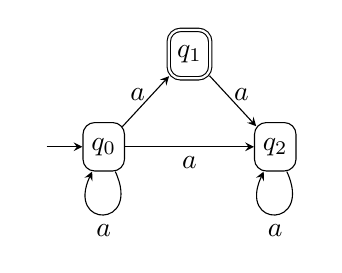
\begin{tikzpicture}[automaton]
\node[state,initial]   (0)                    {\q0};
\node[state,accepting] (1) [above right=of 0] {\q1};
\node[state]           (2) [below right=of 1] {\q2};
\path[->] (0) edge[my below,loop] node[below]           {$a$} ()
              edge[longer1]       node[pos=0.3,above](m){$a$} (1)
              edge                node[below]           {$a$} (2)
          (1) edge[longer1]       node[pos=0.7,above]   {$a$} (2)
          (2) edge[my below,loop] node[below]           {$a$} (); 
\end{tikzpicture}
}

%==============================================================================%
% Michel automata 1 to 4
%==============================================================================%
\newcommand{\labsize}{\scriptsize}  % Size of the edge labels
\newcommand{\MichelOne}{
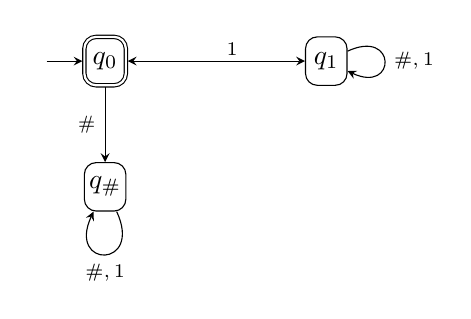
\begin{tikzpicture}[automaton]
% Starting node and # node
\node[state,initial,accepting] (0)               {\q0};
\node[state,yshift=-0.2cm]                   (x) [below=of 0]  {\q\#};
\draw[->] (0) edge node[left] {\labsize\#} (x);
\draw[->] (x) edge[my below,loop] node[below] {\labsize $\#,1$} ();
% Node 1
\node[state,xshift=1.5cm]        (1) [right=of 0]  {\q1};
\draw[<->] (0) edge node[above,xshift=2mm,yshift=-0.5mm] {\labsize $1$} (1);
\draw[->] (1) edge[my right,loop] node[right] {\labsize $\#,1$} ();
\end{tikzpicture}
}

\newcommand{\MichelTwo}{
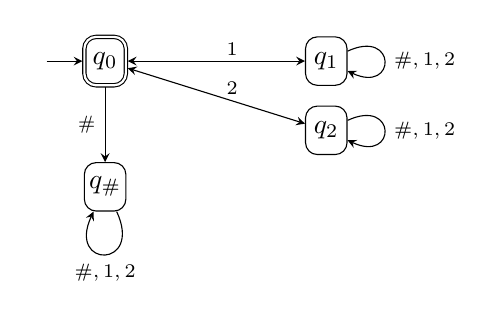
\begin{tikzpicture}[automaton]
% Starting node and # node
\node[state,initial,accepting] (0)               {\q0};
\node[state,yshift=-0.2cm]                   (x) [below=of 0]  {\q\#};
\draw[->] (0) edge node[left] {\labsize\#} (x);
\draw[->] (x) edge[my below,loop] node[below] {\labsize $\#,1,2$} ();
% Node 1
\node[state,xshift=1.5cm]        (1) [right=of 0]  {\q1};
\draw[<->] (0) edge node[above,xshift=2mm,yshift=-0.5mm] {\labsize $1$} (1);
\draw[->] (1) edge[my right,loop] node[right] {\labsize $\#,1,2$} ();
% Node 2
\node[state,yshift=0.5cm]      (2) [below=of 1]  {\q2};
\draw[<->] (0) edge node[above,xshift=2mm,yshift=-1mm] {\labsize $2$} (2);
\draw[->] (2) edge[my right,loop] node[right] {\labsize $\#,1,2$} ();
\end{tikzpicture}
}

\newcommand{\MichelThree}{
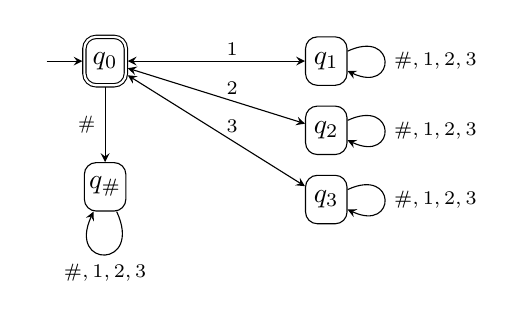
\begin{tikzpicture}[automaton]
% Starting node and # node
\node[state,initial,accepting] (0)               {\q0};
\node[state,yshift=-0.2cm]                   (x) [below=of 0]  {\q\#};
\draw[->] (0) edge node[left] {\labsize\#} (x);
\draw[->] (x) edge[my below,loop] node[below] {\labsize $\#,1,2,3$} ();
% Node 1
\node[state,xshift=1.5cm]        (1) [right=of 0]  {\q1};
\draw[<->] (0) edge node[above,xshift=2mm,yshift=-0.5mm] {\labsize $1$} (1);
\draw[->] (1) edge[my right,loop] node[right] {\labsize $\#,1,2,3$} ();
% Node 2
\node[state,yshift=0.5cm]      (2) [below=of 1]  {\q2};
\draw[<->] (0) edge node[above,xshift=2mm,yshift=-1mm] {\labsize $2$} (2);
\draw[->] (2) edge[my right,loop] node[right] {\labsize $\#,1,2,3$} ();
% Node 3
\node[state,yshift=0.5cm]      (3) [below=of 2]  {\q3};
\draw[<->] (0) edge node[above,xshift=2mm,yshift=-1.5mm] {\labsize $3$} (3);
\draw[->] (3) edge[my right,loop] node[right] {\labsize $\#,1,2,3$} ();
\end{tikzpicture}
}

\newcommand{\MichelFour}{
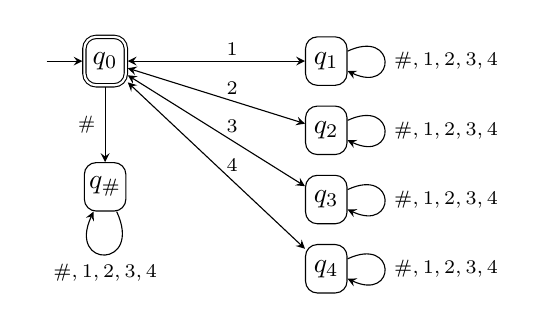
\begin{tikzpicture}[automaton]
% Starting node and # node
\node[state,initial,accepting] (0)               {\q0};
\node[state,yshift=-0.2cm]                   (x) [below=of 0]  {\q\#};
\draw[->] (0) edge node[left] {\labsize\#} (x);
\draw[->] (x) edge[my below,loop] node[below] {\labsize $\#,1,2,3,4$} ();
% Node 1
\node[state,xshift=1.5cm]        (1) [right=of 0]  {\q1};
\draw[<->] (0) edge node[above,xshift=2mm,yshift=-0.5mm] {\labsize $1$} (1);
\draw[->] (1) edge[my right,loop] node[right] {\labsize $\#,1,2,3,4$} ();
% Node 2
\node[state,yshift=0.5cm]      (2) [below=of 1]  {\q2};
\draw[<->] (0) edge node[above,xshift=2mm,yshift=-1mm] {\labsize $2$} (2);
\draw[->] (2) edge[my right,loop] node[right] {\labsize $\#,1,2,3,4$} ();
% Node 3
\node[state,yshift=0.5cm]      (3) [below=of 2]  {\q3};
\draw[<->] (0) edge node[above,xshift=2mm,yshift=-1.5mm] {\labsize $3$} (3);
\draw[->] (3) edge[my right,loop] node[right] {\labsize $\#,1,2,3,4$} ();
% Node 4
\node[state,yshift=0.5cm]      (4) [below=of 3]  {\q4};
\draw[<->] (0) edge node[above,xshift=2mm,yshift=-2mm] {\labsize $4$} (4);
\draw[->] (4) edge[my right,loop] node[right] {\labsize $\#,1,2,3,4$} ();
\end{tikzpicture}
}

%==============================================================================%
% Level symbols for trees and run DAG
%==============================================================================%
\newcommand{\LevelSymbols}{
\begin{tikzpicture}[tree,every tree node/.style={draw=none},edge from parent/.style={draw=none},l/.style={pos=0.3}]
\Tree [ \edge node[l]{$a$}; [ \edge node[l]{$a$}; [ \edge node[l]{$a$}; [ \edge node[l]{$a$}; {} ] ] ] ]
\end{tikzpicture}
}

%==============================================================================%
% Run tree
%==============================================================================%
\newcommand{\RunTree}{
\begin{tikzpicture}[tree]
\Tree
[.\node{\q0}; [.\node{\q0}; [.\node(m){\q0}; [.\node{\q0};    \node{\q0};
                                                              \node[a]{\q1};
                                                              \node{\q2}; ]
                                             [.\node[a]{\q1}; \node{\q2}; ]
                                             [.\node{\q2};    \node{\q2}; ] ]
                            [.\node[a]{\q1}; [.\node{\q2};    \node{\q2}; ] ]
                            [.\node{\q2};    [.\node{\q2};    \node{\q2}; ] ] ]
              [.\node[a]{\q1}; [.\node{\q2}; [.\node{\q2};    \node{\q2}; ] ] ]
              [.\node{\q2}; [.\node{\q2};    [.\node{\q2};    \node{\q2}; ] ] ]]
\node[anchor=base,xshift=-4cm] at (m.base) {$\mathcal{T}^A_{a^\omega}=$};
\end{tikzpicture}
\LevelSymbols
}

%==============================================================================%
% Subset-construction tree
%==============================================================================%
\newcommand{\SubsetConstructionTree}{
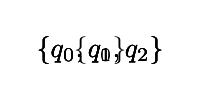
\begin{tikzpicture}[tree]
\Tree
[.\node{\qq0}; [.\node[a]{\qqqq012}; [.\node[a]{\qqqq012}; [.\node[a]{\qqqq012}; \node[a]{\qqqq012}; ] ] ] ]
\end{tikzpicture}
\LevelSymbols
}

%==============================================================================%
% Split tree (left-to-right)
%==============================================================================%
\newcommand{\SplitTreeLeftRight}{
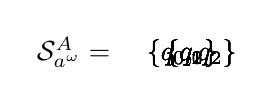
\begin{tikzpicture}[tree]
\Tree
[.\node{\qq0}; [.\node[a]{\qq1};  [.\node(m){\qq2};  [.\node{\qq2};  \node{\qq2}; ] ] ]
              [.\node{\qqq02}; [.\node[a]{\qq1};  [.\node{\qq2};  \node{\qq2}; ] ]
                             [.\node{\qqq02}; [.\node{\qq1};  \node{\qq2}; ]
                                            [.\node{\qqq02}; \node[a]{\qq1};
                                                           \node{\qqq02}; ] ] ] ]
\node[anchor=base,xshift=-1.5cm] at (m.base) {$\mathcal{S}^A_{a^\omega}=$};
\end{tikzpicture}
\LevelSymbols
}

%==============================================================================%
% Split tree (right-to-left)
%==============================================================================%
\newcommand{\SplitTreeRightLeft}{

\begin{tikzpicture}[tree]
\Tree
[.\node{\qq0}; [.\node{\qqq02};  [.\node{\qqq02};  [.\node{\qqq02};  \node{\qqq02};
                                                                     \node[a]{\qq1}; ]
                                                   [.\node[a]{\qq1}; \node{\qq2}; ] ]
                                 [.\node[a]{\qq1}; [.\node{\qq2};    \node{\qq2}; ] ] ]
               [.\node[a]{\qq1}; [.\node{\qq2};    [.\node{\qq2};    \node{\qq2}; ] ] ] ]
\end{tikzpicture}
\LevelSymbols
}

%==============================================================================%
% Reduced split tree left-to-right
%==============================================================================%
\newcommand{\ReducedSplitTreeLeftRight}{
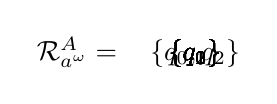
\begin{tikzpicture}[tree]
\Tree
[.\node{\qq0}; [.\node[a]{\qq1}; [.\node(m){\qq2}; [.\node{\qq2}; \node{\qq2}; ] ] ]
               [.\node{\qqq02};    \node[a]{\qq1};
                                 [.\node{\qq0};      \node[a]{\qq1};
                                                   [.\node{\qq0}; \node[a]{\qq1};
                                                            \node{\qq0}; ] ] ] ]
\node[anchor=base,xshift=-1.5cm] at (m.base) {$\mathcal{R}^A_{a^\omega}=$};
\end{tikzpicture}
\LevelSymbols
}

%==============================================================================%
% Reduced split tree right-to-left
%==============================================================================%
\newcommand{\ReducedSplitTreeRightLeft}{
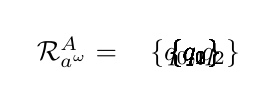
\begin{tikzpicture}[tree]
\Tree
[.\node{\qq0}; [.\node{\qqq02}; [.\node(m){\qq0}; [.\node{\qq0}; \node{\qq0};
                                                            \node[a]{\qq1}; ] 
                                                \node[a]{\qq1}; ]
                               \node[a]{\qq1}; ]
              [.\node[a]{\qq1};  [.\node{\qq2};    [.\node{\qq2}; \node{\qq2}; ] ] ] ]
\node[anchor=base,xshift=-1.5cm] at (m.base) {$\mathcal{R}^A_{a^\omega}=$};
\end{tikzpicture}
\LevelSymbols
}

%==============================================================================%
% Pair of slices of a reduced split tree (right-to-left)
%==============================================================================%
\newcommand{\SlicesOne}{
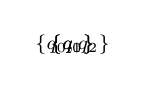
\begin{tikzpicture}[tree,level distance=\myvdistsmall,sibling distance=\myhdistsmall]
\scriptsize
\Tree
[.\node{\qq0}; [.\node   {\qqq02}; ]
               [.\node[a]{\qq1};   ] ] 
\end{tikzpicture}
}

\newcommand{\SlicesTwo}{
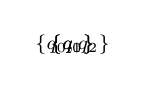
\begin{tikzpicture}[tree,level distance=\myvdistsmall,sibling distance=\myhdistsmall]
\scriptsize
\Tree
[.\node{\qqq02}; [.\node   {\qq0}; ]
                 [.\node[a]{\qq1}; ] ]
\hspace{1.35cm}
\Tree
[.\node[a]{\qq1};   \node{\qq2}; ]
\end{tikzpicture}
}

\newcommand{\SlicesThree}{
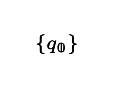
\begin{tikzpicture}[tree,level distance=\myvdistsmall,sibling distance=\myhdistsmall]
\scriptsize
\Tree
[.\node{\qq0}; [.\node   {\qq0}; ]
               [.\node[a]{\qq1}; ] ]
\hspace{1.35cm}
\Tree
[.\node[a]{\qq1}; ]
\hspace{0.9cm}
\Tree
[.\node{\qq2}; \node{\qq2}; ]
\end{tikzpicture}
}

%==============================================================================%
% Run DAG
%==============================================================================%
\newcommand{\RunDAG}{
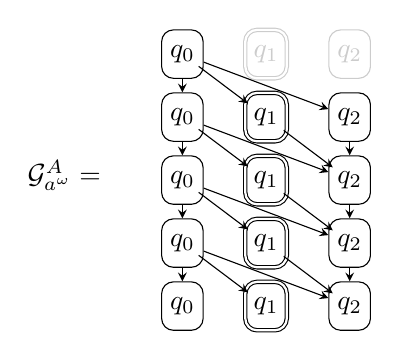
\begin{tikzpicture}[dag]  
\matrix[every node/.style={my state}]{
  \node (00) {\q0}; \& \node[a,ghost] (01) {\q1}; \& \node[ghost] (02) {\q2}; \\
  \node (10) {\q0}; \& \node[a] (11) {\q1}; \& \node (12) {\q2}; \\
  \node (20) {\q0}; \& \node[a] (21) {\q1}; \& \node (22) {\q2}; \\
  \node (30) {\q0}; \& \node[a] (31) {\q1}; \& \node (32) {\q2}; \\
  \node (40) {\q0}; \& \node[a] (41) {\q1}; \& \node (42) {\q2}; \\
};
\path[->]
  (00) edge          (10) edge[longer2] (11) edge (12)
  (10) edge          (20) edge[longer2] (21) edge (22)
  (11) edge[longer2] (22)
  (12) edge          (22)
  (20) edge          (30) edge[longer2] (31) edge (32)
  (21) edge[longer2] (32)
  (22) edge          (32)
  (30) edge          (40) edge[longer2] (41) edge (42)
  (31) edge[longer2] (42)
  (32) edge          (42);  
\node[anchor=base,xshift=-1.5cm] at (20.base) {$\mathcal{G}^A_{a^\omega}=$};      
\end{tikzpicture}
\LevelSymbols
}

%==============================================================================%
% Slices
%==============================================================================%
\newcommand{\Slices}{
%\LevelSymbols
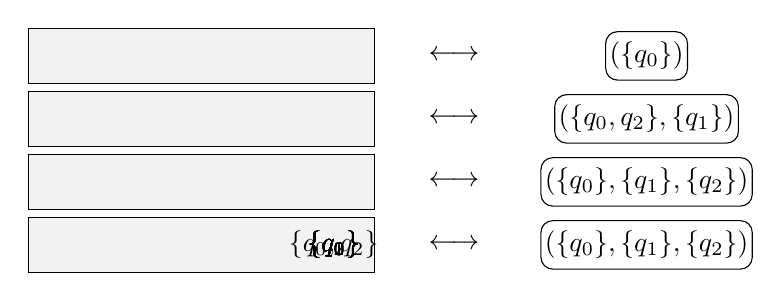
\begin{tikzpicture}[
  tree,
  every tree node/.append style={fill=white},
  automaton,
  frame/.style={
    draw,rectangle,
    minimum width=4.4cm,
    minimum height=2em,
    fill=black!5
  }
]
\Tree
% [.\node{\qq0}; [.\node{\qqq02}; [.\node(m){\qq0}; [.\node{\qq0}; \node{\qq0};
%                                                             \node[a]{\qq1}; ] 
%                                                 \node[a]{\qq1}; ]
%                                \node[a]{\qq1}; ]
%               [.\node[a]{\qq1};  [.\node(m){\qq2};    [.\node{\qq2}; \node{\qq2}; ] ] ] ]
[.\node{\qq0}; [.\node{\qqq02};  [ .\node{\qq0};     \node{\qq0};
                                                     \node[a]{\qq1}; ]
                                   \node[a]{\qq1}; ]
               [.\node[a]{\qq1}; [.\node{\qq2};      \node(m){\qq2}; ] ] ]
\begin{scope}[on background layer]
\node[frame,anchor=east,xshift=0.7mm] (level3) at (m.east) {};
\node[frame,yshift=\myvdist]          (level2) at (level3) {};
\node[frame,yshift=\myvdist]          (level1) at (level2) {};
\node[frame,yshift=\myvdist]          (level0) at (level1) {};
\end{scope}
\begin{scope}[every node/.style={xshift=1cm}]
\node (arrow0) at (level0.east) {$\longleftrightarrow$};
\node (arrow1) at (level1.east) {$\longleftrightarrow$};
\node (arrow2) at (level2.east) {$\longleftrightarrow$};
\node (arrow3) at (level3.east) {$\longleftrightarrow$};
\end{scope}
\begin{scope}[every node/.style={xshift=2cm}]
\node[state] (s0) at (arrow0.east) {$(\qm0)$};
\node[state] (s1) at (arrow1.east) {$(\qqm02,\qm1)$};
\node[state] (s2) at (arrow2.east) {$(\qm0,\qm1,\qm2)$};
\node[state] (s3) at (arrow3.east) {$(\qm0,\qm1,\qm2)$};
\end{scope}
% \path[->] (s0) edge node[right] {$a$} (s1)
%           (s1) edge node[right] {$a$} (s2)
%           (s2) edge[my below,loop] node[below] {$a$} ();
\end{tikzpicture}
}

%==============================================================================%
% Upper part
%==============================================================================%
\newcommand{\UpperPart}{
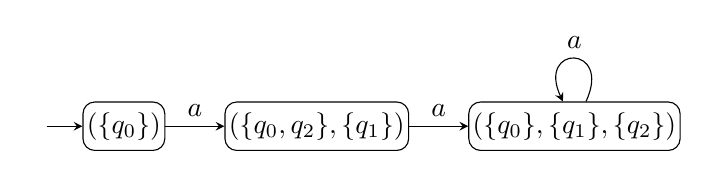
\begin{tikzpicture}[automaton]
\node[state,initial] (0)              {$(\qm0)$};
\node[state]         (1) [right=of 0] {$(\qqm02,\qm1)$};
\node[state]         (2) [right=of 1] {$(\qm0,\qm1,\qm2)$};
\path[->] (0) edge node[above]{$a$} (1)
          (1) edge node[above]{$a$} (2)
          (2) edge[my above,loop] node[above]{$a$} ();
\end{tikzpicture}
}

\newcommand{\UpperPartA}{
\begin{tikzpicture}[automaton,node distance=\myndistsmall]
\scriptsize
\node[state,initial] (0)              {$(\qm0)$};
\begin{scope}[opacity=0]
  \node[state]         (1) [right=of 0] {$(\qqm02,\qm1)$};
  \node[state]         (2) [right=of 1] {$(\qm0,\qm1,\qm2)$};
  \path[->] (0) edge node[above]{$a$} (1)
            (1) edge node[above]{$a$} (2)
            (2) edge[my above,loop] node[above]{$a$} ();
\end{scope}
\end{tikzpicture}
}

\newcommand{\UpperPartB}{
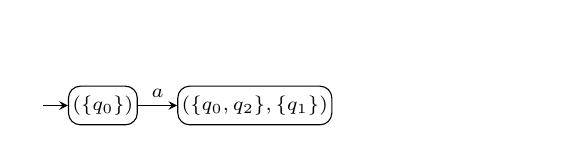
\begin{tikzpicture}[automaton,node distance=\myndistsmall]
\scriptsize
\node[state,initial] (0)              {$(\qm0)$};
\node[state]         (1) [right=of 0] {$(\qqm02,\qm1)$};
\begin{scope}[opacity=0]
  \node[state]         (2) [right=of 1] {$(\qm0,\qm1,\qm2)$};
\end{scope}
\path[->] (0) edge node[above]{$a$} (1);
\begin{scope}[opacity=0]
  \path
            (1) edge node[above]{$a$} (2)
            (2) edge[my above,loop] node[above]{$a$} ();
\end{scope}
\end{tikzpicture}
}

\newcommand{\UpperPartC}{
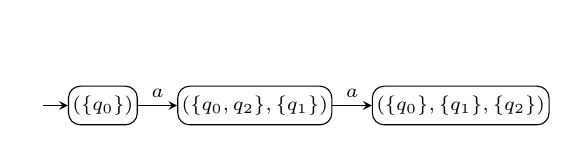
\begin{tikzpicture}[automaton,node distance=\myndistsmall]
\scriptsize
\node[state,initial] (0)              {$(\qm0)$};
\node[state]         (1) [right=of 0] {$(\qqm02,\qm1)$};
\node[state]         (2) [right=of 1] {$(\qm0,\qm1,\qm2)$};
\path[->] (0) edge node[above]{$a$} (1)
          (1) edge node[above]{$a$} (2);
\begin{scope}[opacity=0]
\path 
            (2) edge[my above,loop] node[above]{$a$} ();
\end{scope}
\end{tikzpicture}
}

\newcommand{\UpperPartD}{
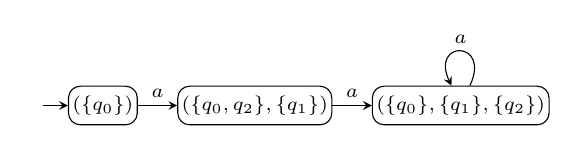
\begin{tikzpicture}[automaton,node distance=\myndistsmall]
\scriptsize
\node[state,initial] (0)              {$(\qm0)$};
\node[state]         (1) [right=of 0] {$(\qqm02,\qm1)$};
\node[state]         (2) [right=of 1] {$(\qm0,\qm1,\qm2)$};
\path[->] (0) edge node[above]{$a$} (1)
          (1) edge node[above]{$a$} (2)
          (2) edge[my above,loop] node[above]{$a$} ();
\end{tikzpicture}
}

%==============================================================================%
% Complement automaton B
%==============================================================================%
\newcommand{\Complement}{
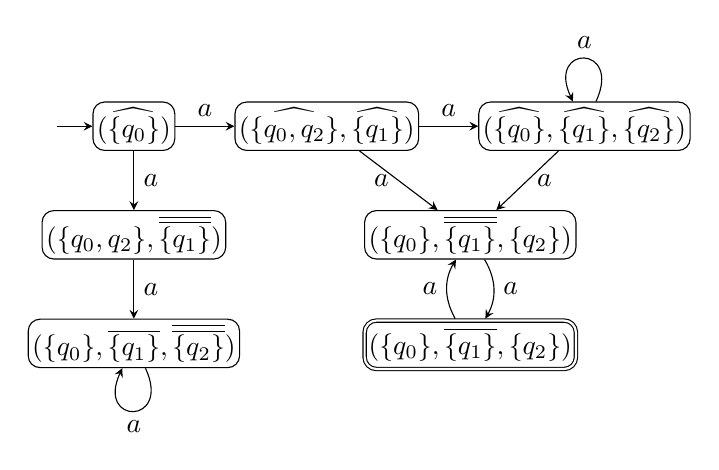
\begin{tikzpicture}[automaton]
\node[state,initial]   (0)               {$(\cl^{\qm0})$};
\node[state]           (1)  [right=of 0] {$(\cl^{\qqm02},\cl^{\qm1})$};
\node[state]           (2)  [right=of 1] {$(\cl^{\qm0},\cl^{\qm1},\cl^{\qm2})$};
\node[state]           (01) [below=of 0] {$(\qqm02,\cl2{\qm1})$};
\node[state,xshift=1cm](11) [right=of 01]{$(\qm0,\cl2{\qm1},\qm2)$};
\node[state]           (02) [below=of 01]{$(\qm0,\cl1{\qm1},\cl2{\qm2})$};
\node[state,accepting] (12) [below=of 11]{$(\qm0,\cl1{\qm1},\qm2)$};
\path[->] (0)  edge                node[above]{$a$} (1)
          (1)  edge                node[above]{$a$} (2)
          (2)  edge[my above,loop] node[above]{$a$} ()
          (0)  edge                node[right]{$a$} (01)
          (01) edge                node[right]{$a$} (02)
          (02) edge[my below,loop] node[below]{$a$} ()
          (1)  edge                node[left] {$a$} (11)
          (11) edge[bend left]     node[right]{$a$} (12)
          (12) edge[bend left]     node[left] {$a$} (11)
          (2)  edge                node[right]{$a$} (11);
\end{tikzpicture}
}

\newcommand{\ComplementA}{
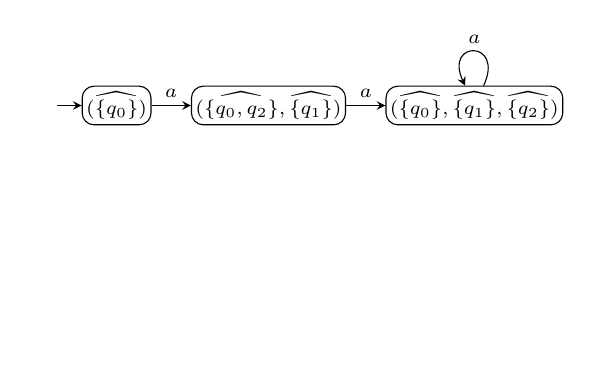
\begin{tikzpicture}[automaton,node distance=\myndistsmall]
\scriptsize
\node[state,initial]   (0)               {$(\cl^{\qm0})$};
\node[state]           (1)  [right=of 0] {$(\cl^{\qqm02},\cl^{\qm1})$};
\node[state]           (2)  [right=of 1] {$(\cl^{\qm0},\cl^{\qm1},\cl^{\qm2})$};
\begin{scope}[opacity=0]
  \node[state]           (01) [below=of 0] {$(\qqm02,\cl2{\qm1})$};
  \node[state,xshift=1cm](11) [right=of 01]{$(\qm0,\cl2{\qm1},\qm2)$};
  \node[state]           (02) [below=of 01]{$(\qm0,\cl1{\qm1},\cl2{\qm2})$};
  \node[state,accepting] (12) [below=of 11]{$(\qm0,\cl1{\qm1},\qm2)$};
\end{scope}
\path[->] (0)  edge                node[above]{$a$} (1)
          (1)  edge                node[above]{$a$} (2)
          (2)  edge[my above,loop] node[above]{$a$} ();
\begin{scope}[opacity=0]
  \path
            (0)  edge                node[right]{$a$} (01)
            (01) edge                node[right]{$a$} (02)
            (02) edge[my below,loop] node[below]{$a$} ()
            (1)  edge                node[left] {$a$} (11)
            (11) edge[bend left]     node[right]{$a$} (12)
            (12) edge[bend left]     node[left] {$a$} (11)
            (2)  edge                node[right]{$a$} (11);
\end{scope}
\end{tikzpicture}
}

\newcommand{\ComplementB}{
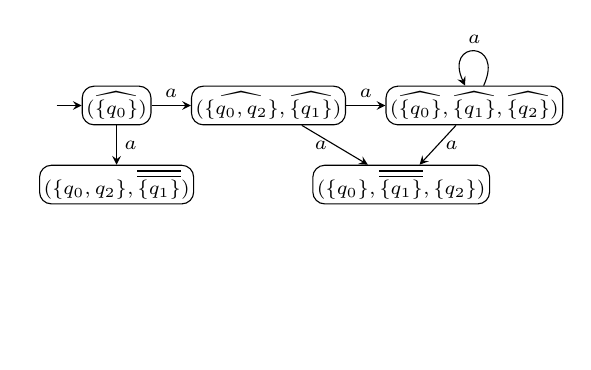
\begin{tikzpicture}[automaton,node distance=\myndistsmall]
\scriptsize
\node[state,initial]   (0)               {$(\cl^{\qm0})$};
\node[state]           (1)  [right=of 0] {$(\cl^{\qqm02},\cl^{\qm1})$};
\node[state]           (2)  [right=of 1] {$(\cl^{\qm0},\cl^{\qm1},\cl^{\qm2})$};
\node[state]           (01) [below=of 0] {$(\qqm02,\cl2{\qm1})$};
\node[state,xshift=1cm](11) [right=of 01]{$(\qm0,\cl2{\qm1},\qm2)$};
\begin{scope}[opacity=0]
  \node[state]           (02) [below=of 01]{$(\qm0,\cl1{\qm1},\cl2{\qm2})$};
  \node[state,accepting,opacity=0] (12) [below=of 11]{$(\qm0,\cl1{\qm1},\qm2)$};
\end{scope}
\path[->] (0)  edge                node[above]{$a$} (1)
          (1)  edge                node[above]{$a$} (2)
          (2)  edge[my above,loop] node[above]{$a$} ()
          (0)  edge                node[right]{$a$} (01)
          (1)  edge                node[left] {$a$} (11)
          (2)  edge                node[right]{$a$} (11);
\begin{scope}[opacity=0]
  \path
            (01) edge                node[right]{$a$} (02)
            (02) edge[my below,loop] node[below]{$a$} ()
            (11) edge[bend left]     node[right]{$a$} (12)
            (12) edge[bend left]     node[left] {$a$} (11);
\end{scope}
\end{tikzpicture}
}

\newcommand{\ComplementC}{
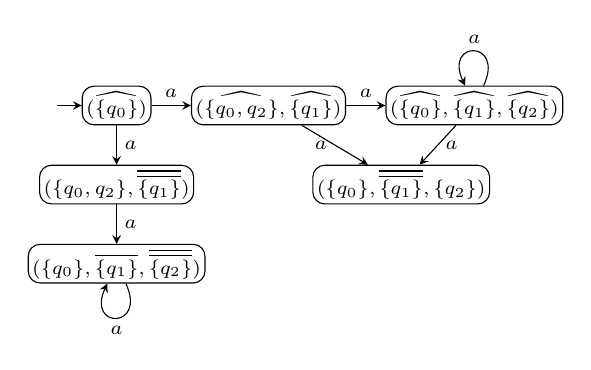
\begin{tikzpicture}[automaton,node distance=\myndistsmall]
\scriptsize
\node[state,initial]   (0)               {$(\cl^{\qm0})$};
\node[state]           (1)  [right=of 0] {$(\cl^{\qqm02},\cl^{\qm1})$};
\node[state]           (2)  [right=of 1] {$(\cl^{\qm0},\cl^{\qm1},\cl^{\qm2})$};
\node[state]           (01) [below=of 0] {$(\qqm02,\cl2{\qm1})$};
\node[state,xshift=1cm](11) [right=of 01]{$(\qm0,\cl2{\qm1},\qm2)$};
\node[state]           (02) [below=of 01]{$(\qm0,\cl1{\qm1},\cl2{\qm2})$};
\begin{scope}[opacity=0]
  \node[state,accepting,opacity=0] (12) [below=of 11]{$(\qm0,\cl1{\qm1},\qm2)$};
\end{scope}
\path[->] (0)  edge                node[above]{$a$} (1)
          (1)  edge                node[above]{$a$} (2)
          (2)  edge[my above,loop] node[above]{$a$} ()
          (0)  edge                node[right]{$a$} (01)
          (1)  edge                node[left] {$a$} (11)
          (2)  edge                node[right]{$a$} (11)
          (01) edge                node[right]{$a$} (02)
          (02) edge[my below,loop] node[below]{$a$} ();
\begin{scope}[opacity=0]
  \path
            (11) edge[bend left]     node[right]{$a$} (12)
            (12) edge[bend left]     node[left] {$a$} (11);
\end{scope}
\end{tikzpicture}
}

\newcommand{\ComplementD}{
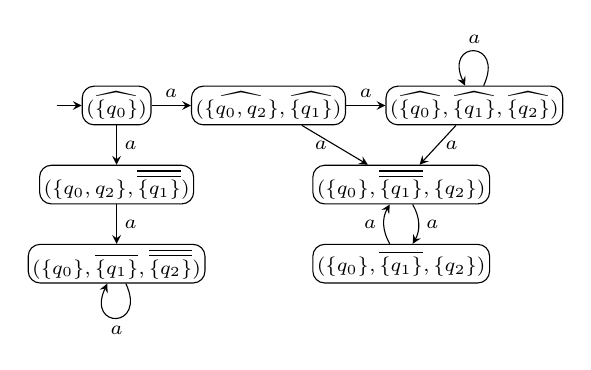
\begin{tikzpicture}[automaton,node distance=\myndistsmall]
\scriptsize
\node[state,initial]   (0)               {$(\cl^{\qm0})$};
\node[state]           (1)  [right=of 0] {$(\cl^{\qqm02},\cl^{\qm1})$};
\node[state]           (2)  [right=of 1] {$(\cl^{\qm0},\cl^{\qm1},\cl^{\qm2})$};
\node[state]           (01) [below=of 0] {$(\qqm02,\cl2{\qm1})$};
\node[state,xshift=1cm](11) [right=of 01]{$(\qm0,\cl2{\qm1},\qm2)$};
\node[state]           (02) [below=of 01]{$(\qm0,\cl1{\qm1},\cl2{\qm2})$};
\node[state]           (12) [below=of 11]{$(\qm0,\cl1{\qm1},\qm2)$};
\path[->] (0)  edge                node[above]{$a$} (1)
          (1)  edge                node[above]{$a$} (2)
          (2)  edge[my above,loop] node[above]{$a$} ()
          (0)  edge                node[right]{$a$} (01)
          (01) edge                node[right]{$a$} (02)
          (02) edge[my below,loop] node[below]{$a$} ()
          (1)  edge                node[left] {$a$} (11)
          (11) edge[bend left]     node[right]{$a$} (12)
          (12) edge[bend left]     node[left] {$a$} (11)
          (2)  edge                node[right]{$a$} (11);
\end{tikzpicture}
}

%==============================================================================%
% Run types
%==============================================================================%
\newcommand{\RunTypes}{
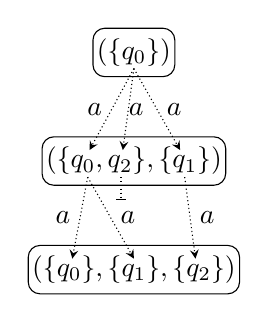
\begin{tikzpicture}[automaton]
\node[state] (0)              {$(\qm0)$};
\node[state] (1) [below=of 0] {$(\qqm02,\qm1)$};
\node[state] (2) [below=of 1] {$(\qm0,\qm1,\qm2)$};
\path[->,densely dotted]
($(0.south)+(0,1.1mm)$)
    edge node[right]     {$a$} ($(1.north east)!0.25!(1.north west)-(0,1.75mm)$)
    edge node[xshift=1mm]{$a$} ($(1.north east)!0.56!(1.north west)-(0,1.75mm)$)
    edge node[left]      {$a$} ($(1.north east)!0.74!(1.north west)-(0,1.75mm)$)
($(1.south east)!0.225!(1.south west)+(0,1.1mm)$)
    edge node[right]{$a$} ($(2.north east)!0.21!(2.north west)-(0,1.75mm)$)
($(1.south east)!0.75!(1.south west)+(0,1.1mm)$)
    edge node[right]{$a$} ($(2.north east)!0.50!(2.north west)-(0,1.75mm)$)
    edge node[left] {$a$} ($(2.north east)!0.79!(2.north west)-(0,1.75mm)$);
\draw[-{Bar[width=1.25mm]},densely dotted]
    ($(1.south east)!0.57!(1.south west)+(0,1.1mm)$) --
    ($(1.south east)!0.57!(1.south west)-(0,1.8mm)$);
\end{tikzpicture}
\hfil
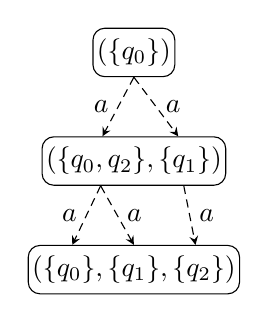
\begin{tikzpicture}[automaton]
\node[state] (0)              {$(\qm0)$};
\node[state] (1) [below=of 0] {$(\qqm02,\qm1)$};
\node[state] (2) [below=of 1] {$(\qm0,\qm1,\qm2)$};
\path[->,densely dashed]
(0.south)
    edge node[right]{$a$} ($(1.north east)!0.26!(1.north west)$)
    edge node[left] {$a$} ($(1.north east)!0.67!(1.north west)$)
($(1.south east)!0.23!(1.south west)$)
    edge node[right]{$a$} ($(2.north east)!0.21!(2.north west)$)
($(1.south east)!0.68!(1.south west)$)
    edge node[right]{$a$} ($(2.north east)!0.50!(2.north west)$)
    edge node[left] {$a$} ($(2.north east)!0.79!(2.north west)$);
\end{tikzpicture}
\hfil
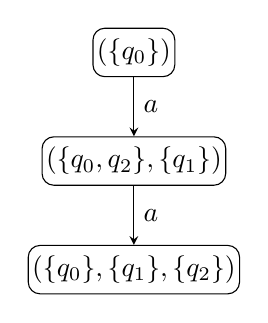
\begin{tikzpicture}[automaton]
\node[state] (0)              {$(\qm0)$};
\node[state] (1) [below=of 0] {$(\qqm02,\qm1)$};
\node[state] (2) [below=of 1] {$(\qm0,\qm1,\qm2)$};
\path[->] (0) edge node[right]{$a$} (1)
          (1) edge node[right]{$a$} (2);
\end{tikzpicture}
}

%==============================================================================%
% Expressive equivalences
%==============================================================================%
\newcommand{\Equivalences}{
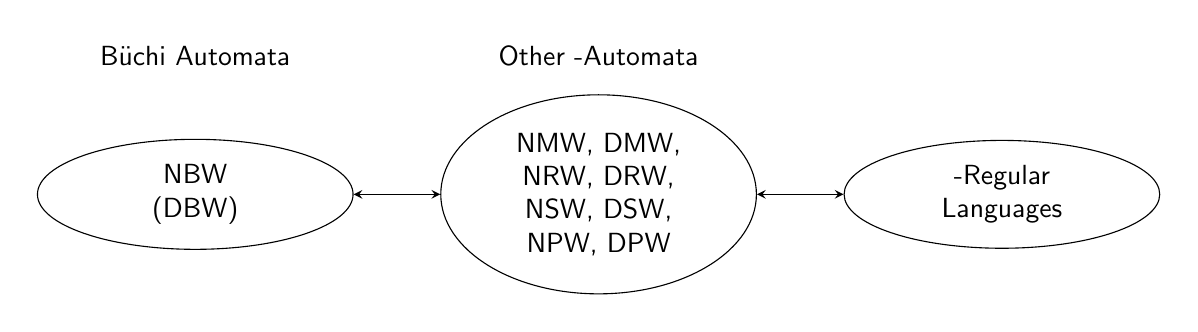
\begin{tikzpicture}[mtrx,s/.style={ellipse,draw,text width=2.6cm,align=center}]
\matrix[column sep=1.1cm,row sep=0.25cm]{
  \node               {Büchi Automata}; \& 
  \node               {Other \om-Automata}; \&
  \\
  \node[s] (left)   {NBW\\(DBW)}; \& 
  \node[s] (middle) {NMW, DMW,\\NRW, DRW,\\NSW, DSW,\\NPW, DPW}; \& 
  \node[s] (right)  {\om-Regular\\Languages}; \\
};
\path[<->] (left)   edge (middle)
           (middle) edge (right);
\end{tikzpicture}
}

%==============================================================================%
% Complementation construction
%==============================================================================%
\newcommand{\Complementation}{

\begin{tikzpicture}[box/.style={text width=2.5cm,align=center}]
\node[box]      (l)              {Büchi Automaton $A$};
\node[draw,box] (m) [right=of l] {Complementation construction};
\node[box]      (r) [right=of m] {Büchi automaton $B$\\$L(B) = \cl1{L(A)}$}; 
\path[->] (l) edge (m)
          (m) edge (r);
\end{tikzpicture}
}
